\section{Visualisation}
The final implementation stage was the visualisation of the results. To ensure 
that the visualisation was not tightly coupled to the analysis process, the 
visualisation aspect had been specifically kept as a separate entity.

The reason for this is that it allows BlackBerry to develop their own 
visualisation techniques if required, without having to change the main 
analysis processes.

\subsection{Data Management}
To ensure that the visualisation is loosely coupled with the analysis part of 
the tool, a simple data structure was required to be implemented.

As the charts were to be developed using web technologies (such as HTML, CSS 
and JavaScript), it made sense to maintain the data structures in JavaScript 
Object Notation (JSON), which is what the tool outputs.

\subsection{Charts}
In order to produce some visualisation charts, a JavaScript charting library is
required. The decision to use a well established charting library, rather than 
developing one from scratch was suggested by BlackBerry.

The requirement to develop visualisation charts was only identified as a 
`could' requirement (see section \ref{sec:could}). However due to time 
resourcing being managed well, this requirement could be fulfilled.

The charting library that was selected is call d3js. D3js is a ``JavaScript 
library for manipulating documents based on data'' \citep{d3js}. One of the 
major advantages for using d3js is that it is based upon open, standard web 
technologies (HTML, DOM, CSS and JavaScript).

This effectively means that the resulting output will be able to be displayed 
on almost any computer, without the requirement for additional software to be
installed --- other than a web standard browser.

Five charting techniques were selected to output the data, and are described in
more detail in the following subsections.


\subsubsection{Bar Chart}
The Bar Chart is one of the main points of entry to analyse the results. The 
raw data is arranged in a hierarchical structure, and this is something that 
the Bar Chart supports.

Figure \ref{fig:bar_chart_1} highlights an example bar chart from an initial 
point of view.

A user is able to ``drill down'' into the data to find specific information, by
simply clicking upon a given bar. Figure \ref{fig:bar_chart_2} highlights all 
the clusters whereby the 9800 device dropped calls upon a specific RAT. 

Clicking upon one of the bars again will drill down into the specifics of a 
cluster.

\afterpage{
  % Flush earlier floats (otherwise order might not be correct)
  \clearpage
  % empty page style (?)
  %\thispagestyle{empty}
  % Landscape page
  \begin{landscape}
    % Center image
    \centering 
      \begin{figure}[H]
        \centering
          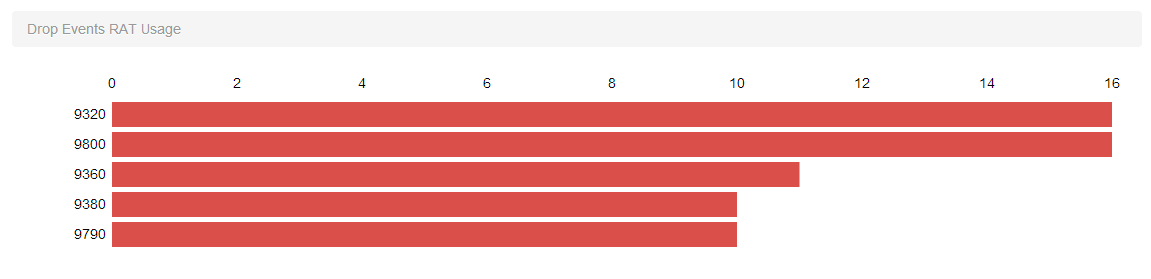
\includegraphics[scale=0.75]{chapter8/visualisation/bar_chart_1.png}
          \caption[Example Bar Chart output]
                  {An Example Bar Chart output from the root node, highlighting all 
                   the various devices and their performance from a general point of 
                   view}
          \label{fig:bar_chart_1}
      \end{figure}
      ~\\
      \begin{figure}[H]
        \centering
          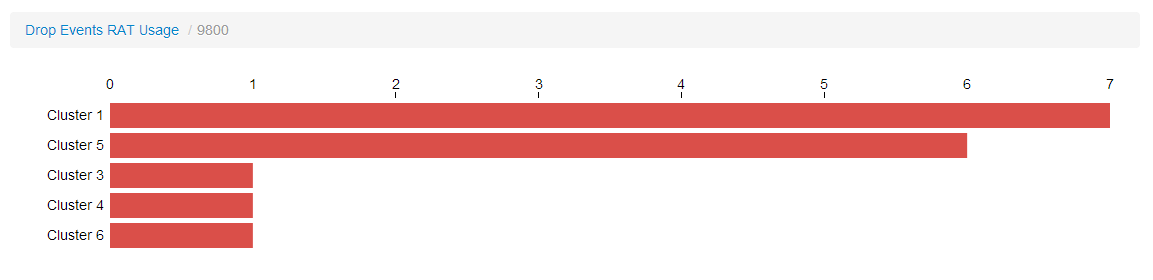
\includegraphics[scale=0.75]{chapter8/visualisation/bar_chart_2.png}
          \caption[Example Bar Chart output one node deep]
                  {Example Bar Chart output one node deep --- i.e. all data that is
                   related to the 9800 device only.}
          \label{fig:bar_chart_2}
      \end{figure}

  \end{landscape}
  % Flush page
  \clearpage
}


\newpage
\subsubsection{Circle Pack}
A Circle Pack diagram represent hierarchy through the use of embedded nodes. 
A Circle Pack diagram can be compared to a treemap, as it shares similar 
features however it is not as space-efficient. 

On the other hand it does reveal the overall size of each element (cluster, 
device, week, usage) more vividly in comparison to a treemap. Figure 
\ref{fig:circle_pack} illustrates an example output.

\afterpage{
  % Flush earlier floats (otherwise order might not be correct)
  \clearpage
  % empty page style (?)
  %\thispagestyle{empty}
  % Landscape page
  \begin{landscape}
    % Center image
    \centering 

      \begin{figure}[H]
        \centering
          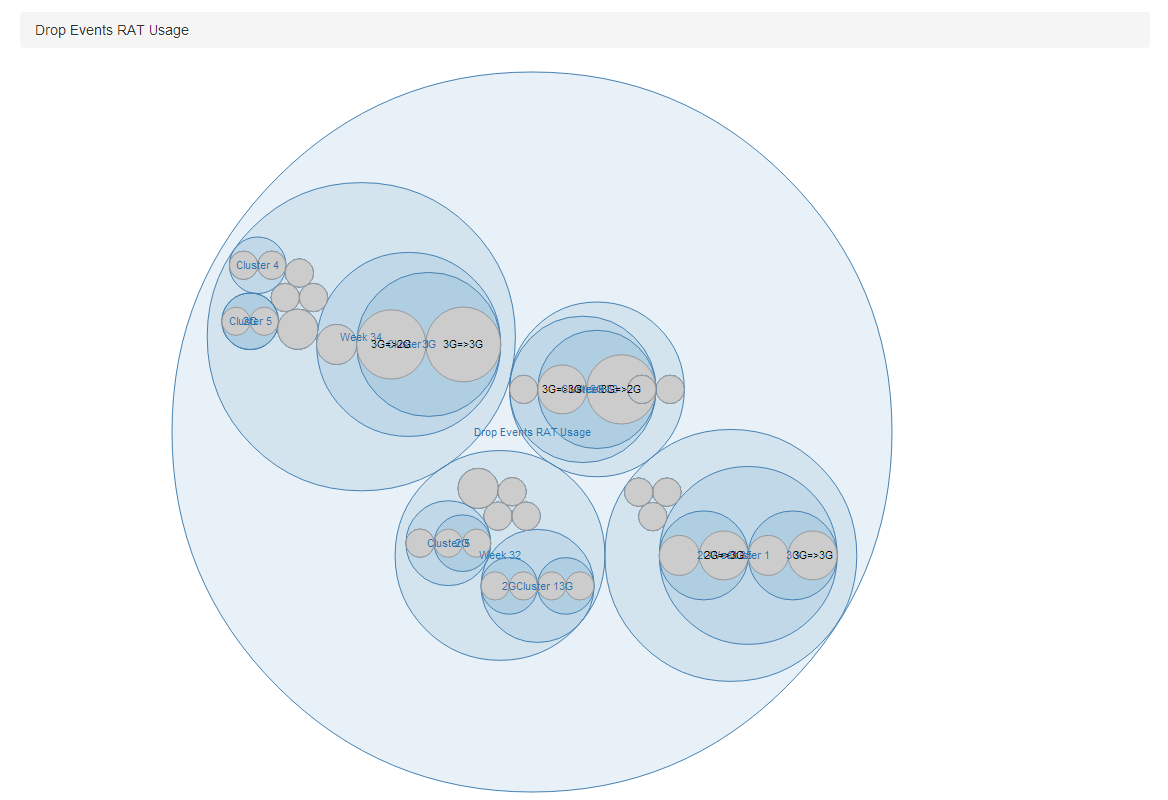
\includegraphics[scale=0.70]{chapter8/visualisation/circle_pack.png}
          \caption[Example Circle Pack output]
                  {Example Circle Pack output, highlighting all the nodes. The 
                  first node is the week, e.g. week 34.}
          \label{fig:circle_pack}
      \end{figure}

  \end{landscape}
  % Flush page
  \clearpage
}


\newpage
\subsubsection{Dendrogram}

** IMAGE **



\newpage
\subsubsection{Partition Chart}
A partition chart can thought of as an alternative to a pie chart. Although it 
looks more like a treemap, it more closely resembles the characteristics of a 
pie chart.

As with the previous charts, the partition chart supports hierarchical data. 
This allows the user to click upon a given area, and the chart will rearrange 
itself. This allows for a more bespoke, ``drilled down'' view to viewing the 
analysis.

Figure \ref{fig:partition_chart} highlights an example partition chart.

\begin{figure}[H]
  \centering
    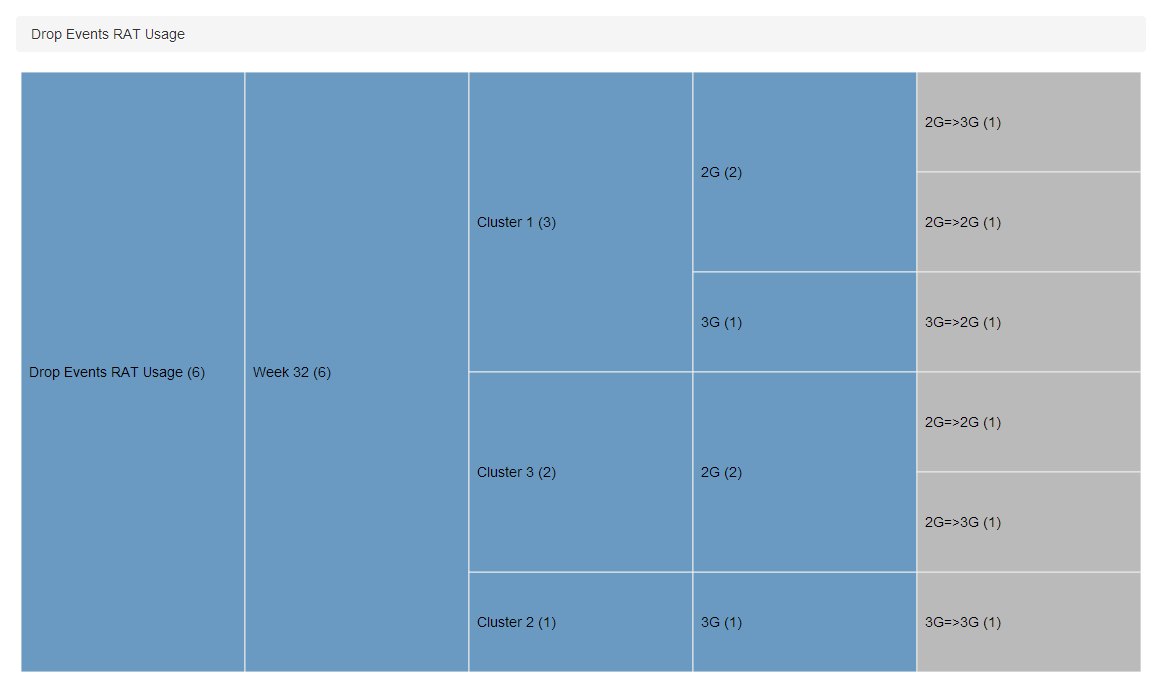
\includegraphics[scale=0.55]{chapter8/visualisation/partition.png}
    \caption[Example Partition output]
            {Example Partition output, highlighting all the nodes for the drop 
             events usage figures.}
    \label{fig:partition_chart}
\end{figure}


\newpage
\subsubsection{Treemap}
A treemap illustrates data as a set of nested rectangles. Like the partition 
chart, treemaps support hierarchical data structures.

Each square represents the total count of the events --- the larger the square 
the more events were found with the criteria. As with the partition chart, 
patterns within the data can be easily spotted. 

As a treemap grows, the efficiently of the use of space will also grow. The 
treemap implementation allows for a user to click upon a square, and it will 
rearrange itself, and as with many other charts will allow for a ``drilled 
down'' view.

Figure \ref{fig:treemap} highlights an example treemap.

\begin{figure}[H]
  \centering
    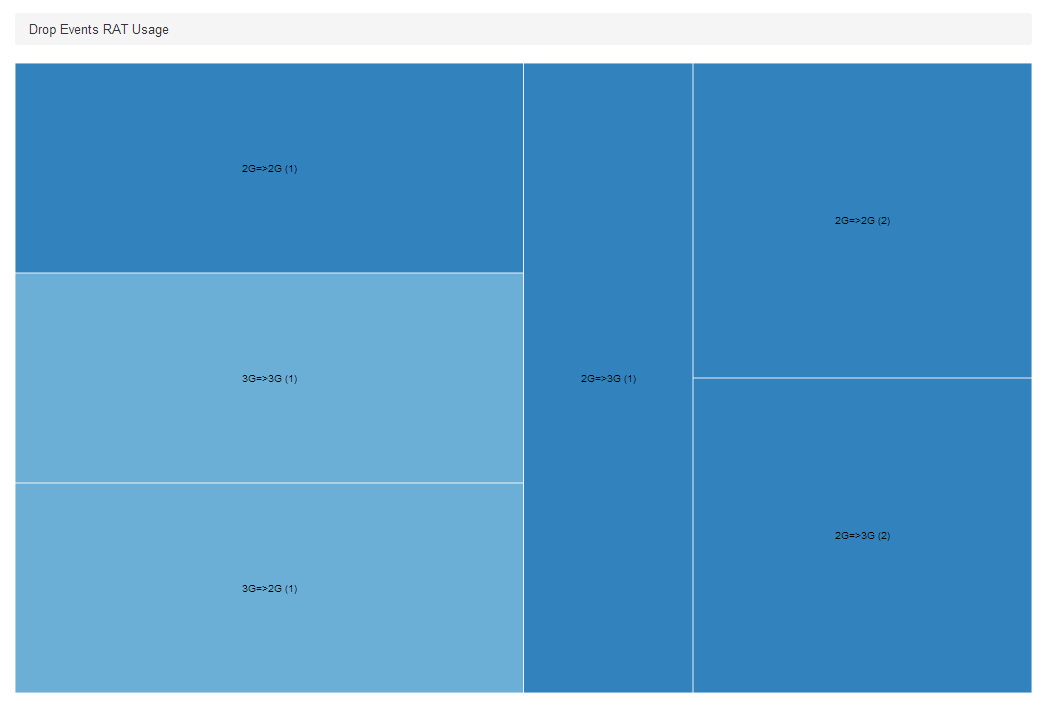
\includegraphics[scale=0.60]{chapter8/visualisation/treemap.png}
    \caption[Example Treemap output]
            {Example Treemap output, highlighting all the nodes for the drop 
             events usage figures.}
    \label{fig:treemap}
\end{figure}